\documentclass[conference]{IEEEtran}
\usepackage{amsmath,amssymb}
\usepackage{graphicx}
\usepackage{booktabs}
\usepackage{hyperref}
\usepackage{cite}

% Standard, content-neutral space tightening (whitespace only, no text/citation changes):
\setlength{\textfloatsep}{6pt plus 1pt minus 1pt}
\setlength{\intextsep}{6pt plus 1pt minus 1pt}
\setlength{\floatsep}{4pt plus 1pt minus 1pt}
\setlength{\abovecaptionskip}{3pt}
\setlength{\belowcaptionskip}{2pt}
\renewcommand{\IEEEbibitemsep}{0pt plus .3pt}

\begin{document}

\title{When Do Music Graphs Matter?\\
A Four-Task Study of Text, Structure, Fusion, and Cross-Modal Retrieval}

\author{
\IEEEauthorblockN{Nazmul Islam, Md. Khaliduzzaman Khan Samrat, Atanu Roy}
\IEEEauthorblockA{BRAC University\\
nazmul.islam1@bracu.ac.bd, md.khaliduzzaman@bracu.ac.bd, atanu.roy@bracu.ac.bd}
}

\maketitle

\begin{abstract}
Music understanding systems often combine text and audio, and audio is often represented as
a graph: short segments become nodes, with edges linking segments close in time or similar
in content. When a graph's structure is a deterministic function of its own node features,
the data-processing inequality guarantees it cannot add Shannon information beyond those
features -- an analytic fact, not something an experiment can test. What experiments can
test is the practical question: whether such a graph still helps a real, finite model, e.g.\
as a computational shortcut or inductive bias. We test this directly across four tasks
sharing the same node features and graph construction rule: text-only tag prediction,
graph-based genre classification, graph-plus-text fusion, and audio-text contrastive
retrieval. Tasks 2 and 4 each compare their graph-based model against a width/depth-matched,
lower-parameter edge-free alternative on held-out test data; Task 3's own comparison is
validation-only, so its evidence comes from two test-set diagnostics instead:
branch-zeroing inside the trained fusion model, and a cross-tabulation of
independently-trained single-branch checkpoints. No task shows a graph-based model with a
\emph{learned} aggregation step clearly ahead of its edge-free counterpart -- though a
non-learned exact 2-hop aggregation in genre classification outperforms both, using a
different training recipe than what it is compared against, so this suggests
under-exploited topology, not a clean ablation (reported, not hidden). In fusion, zeroing
the graph branch changes only 1.7\% of individual predictions and costs 0.009 macro-F1 --
small, not zero. A complementarity check first appears to show the graph-only model
correcting 48.5\% of the text-only model's errors, but splitting by label polarity shows it
predicts a tag present at all for only 5 of 50 tags, and fewer than 1\% of its apparent
corrections are genuine detections -- not real complementary signal as originally framed; a
follow-up check in a second implementation did not confirm this reading, discussed rather
than resolved. In retrieval, graph-based and no-graph encoders show no reliable difference
across three seeds, on every metric. We also checked two alternative explanations rather
than assume them away: caption text leaking target labels directly (it does,
substantially), and duplicate audio between train and test in one dataset (real, confirmed
for a small number of tracks, left open as an unresolved caveat for the smallest
comparison). We do not conclude graphs are useless for music -- only that this specific
construction does not reliably help beyond its own node features, for these tasks, on
these datasets. We report this as the paper's central finding, not a failed architecture
search.
\end{abstract}

\section{Introduction}

Music understanding systems increasingly combine several kinds of input: a natural-language
description of a track, and the track's own audio. Audio is often turned into a graph before
it reaches a model -- a track is split into short segments, each becomes a node, and edges
connect segments close in time or acoustically similar. This is a reasonable design choice:
music has real relational structure (repetition, transition, similarity between sections),
and a graph neural network (GNN) can in principle use it. Similarity between short audio
segments, computed from acoustic features and thresholded or visualized as a matrix, is a
long-established technique for finding structure within a track \cite{foote2000novelty};
this paper's graph construction applies the same idea (pairwise segment similarity) to build
a graph rather than a novelty curve. The message-passing GNN family this paper draws its
encoder from includes several related architectures beyond the one used here -- GCN
\cite{kipf2017gcn}, GAT \cite{velickovic2018gat}, and GIN \cite{xu2019gin}, alongside
GraphSAGE \cite{hamilton2017graphsage}. Separately, a recognized concern in the broader GNN
literature is that graph-based models are not always compared against simpler baselines
under matched, controlled conditions \cite{errica2020fair,shchur2018pitfalls} -- this paper
takes that concern as a direct methodological starting point, not only a citation.

But if the edges are built directly from the same features already given to each node --
connecting two segments whenever their feature similarity crosses a threshold -- then the
graph's structure is, information-theoretically, a restatement of information already
present in the node features, not a new observation about the track. This does not
automatically mean such a graph is useless: a deterministic function of the features could
still act as a useful computational shortcut or inductive bias, easing optimization even
without adding information a sufficiently powerful model could not already extract from the
features alone. Whether either possibility -- added information, or a
useful-but-informationless shortcut -- actually helps in practice, for a specific
construction and specific tasks, is an empirical question, not something to assume from the
architecture diagram alone.

This paper answers that question for one concrete system, across four tasks sharing the same
node-feature definition and similarity-based edge construction rule -- though not, as
Section~\ref{sec:data} discloses precisely, the same audio segmentation length or dataset
split in every task: a text-only tag classifier (Task 1, no audio at all), a graph-based
genre classifier compared against an edge-free alternative (Task 2), a graph-plus-text fusion
model (Task 3), and a contrastive audio-text retrieval model (Task 4). Each task, alone,
answers a narrower question. Together, they form a single experimental ladder:

\begin{itemize}
\item \textbf{Task 1} asks how much target information language alone already provides,
before any audio or graph is involved.
\item \textbf{Task 2} asks whether the graph's topology helps audio-only classification
beyond what the same node features give a structure-free model.
\item \textbf{Task 3} asks whether the graph adds information that a strong text model does
not already have, once both are available together.
\item \textbf{Task 4} asks whether any graph benefit found in classification or fusion
survives under a different objective entirely: matching audio to text by similarity, with no
genre or tag labels -- only audio-caption pairing as supervision.
\end{itemize}

We do not set out to show that graphs are useless for music, and we do not find that. We set
out to check, directly and with matched controls wherever they could be arranged --
Section~\ref{sec:protocol} discloses the specific exceptions found on inspection, including
one confound in Task 2's own training scripts -- whether \emph{this} similarity-based graph
construction earns its place in \emph{these} tasks. Task 1 has no graph and serves as the
anchor; Tasks 2--4 each include a direct graph-vs-edge-free comparison, and in none does the
graph-based model come out clearly and reliably ahead. Task 2's fairest (pooling-matched)
comparison favors the edge-free alternative, though a non-learned 2-hop control complicates
this (Section~\ref{sec:discussion}). Task 3's standalone comparison is mixed and
inconclusive, but its two follow-up diagnostics tell distinct, narrower stories:
branch-zeroing (an inference-time intervention on the trained fusion model) finds it relies
only slightly on the graph branch -- topology and node features together, not
topology-isolating -- while complementarity (correlational, comparing two separately-trained
models rather than probing the fusion model) finds almost no positive-label rescue by the
graph-only model, no sign it detects tags text misses. Together, in this evidence base, they
point toward little demonstrated graph value for Task 3, though neither is topology-isolating
and complementarity says nothing about the fusion model's own behavior; a follow-up check in
a second implementation did not confirm even this narrower reading, reported openly in
Section~\ref{sec:discussion} rather than alongside only the reading that fits. Task 4 shows
no consistent advantage either way across three seeds. We report this consistency, with each
result's own caveats, as the paper's main finding. We also check two alternative explanations
that could produce this pattern without the graph itself being at fault -- caption text
directly leaking target labels, and duplicate or leaked audio inflating a model's score --
and report what we find, rather than assume either away.

\section{Four-Task Study Design}\label{sec:design}

The four tasks are not identical in dataset, label space, objective, or metric -- Task 1 has
no graph at all, Task 2 is single-label classification on GTZAN, Task 3 is multi-label
classification on MusicCaps, and Task 4 is a ranking objective with no genre or tag class
labels, using audio-caption pair identity as supervision. What they do
share is the node-feature definition (32-dimensional chroma plus MFCC), the same
similarity-based graph construction rule, and closely matched encoder architectures where a
graph is involved; Task 4 was also built in a separate implementation with a different
segment length and dataset split (Section~\ref{sec:data} discloses this precisely). This
shared representation is what makes a cross-task comparison informative at all: each task's
own graph-vs-edge-free result is its own self-contained comparison, with its own explicitly
disclosed matching exceptions (Section~\ref{sec:protocol}) rather than a uniform fairness
guarantee across tasks, and it
is the \emph{consistency of the overall conclusion} those results support -- not an
identical numeric comparison in every task, and not an assumption that every task used
byte-identical inputs -- that the cross-task analysis in Section~\ref{sec:cross-task} relies
on.

\textbf{Task 1 -- Text Tag Prediction.} A text-only reference point. A BERT-family encoder
predicts tags from a caption alone, with no audio and no graph at all. This establishes how
much of the target signal language already carries by itself -- a qualitative anchor for the
rest of the paper's "does the graph add anything" question, not a numerical baseline every
later task's own metric is scored against, since Task 2 uses a different dataset and label
space and Task 4 uses a different metric entirely.

\textbf{Task 2 -- Graph-Based Audio Classification.} A graph neural network predicts genre
from an audio-only segment graph, compared against (a) a non-graph CNN baseline operating
directly on the log-mel spectrogram, and (b) a width/depth-matched, lower-parameter, edge-free
encoder using the exact same node features as the graph model, with every edge removed.
Comparison (b) tests whether the graph encoder, as a whole, adds anything over a
structure-free alternative; because it changes the aggregation operator along with the
edges, it does not isolate topology alone -- Section~\ref{sec:results-t2} also reports a
same-architecture, edges-only intervention from a companion audit for that narrower
question.

\textbf{Task 3 -- Multimodal Context Prediction.} A graph encoder of the same architecture as
Task 2's is fused with a separately initialized instance of the same pretrained text-encoder
architecture used in Task 1 (not Task 1's own trained weights), compared across four fusion
strategies (text-only, graph-only,
concatenation, cross-attention) plus two diagnostics: zeroing the graph branch inside a
trained fusion model, and cross-tabulating which examples the text-only and graph-only
models get right or wrong. This tests whether the graph is complementary to text, not just
whether it is useful on its own.

\textbf{Task 4 -- Audio-Text Retrieval.} A contrastive dual encoder learns to match a
caption to its audio clip, with no genre or tag class labels, using only audio-caption
pairing as supervision -- a different objective from classification,
scored by ranking (Recall@K) rather than accuracy. The same graph-vs-edge-free comparison
from Task 2 is repeated here, to test whether any graph advantage (or its absence) generalizes
beyond classification to a fundamentally different task type.

Figure~\ref{fig:progression} summarizes the ladder: each task adds one element -- audio,
fusion, then a different objective -- while keeping the node-feature definition and graph
construction rule fixed (Section~\ref{sec:data} discloses where the underlying
implementation still differs between tasks).

\begin{figure}[t]
\centering
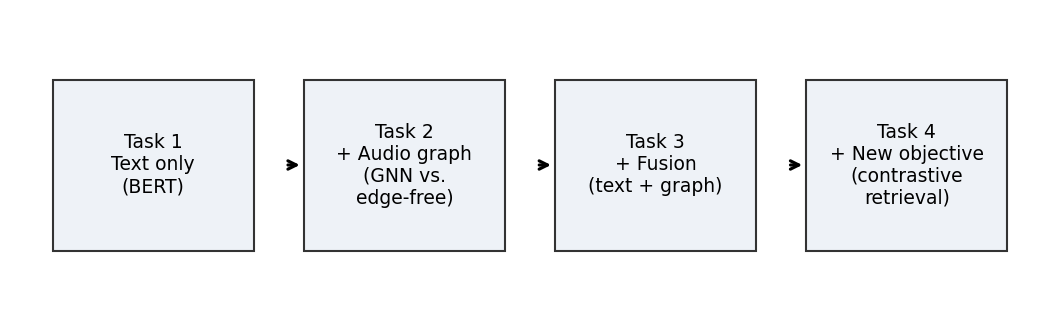
\includegraphics[width=0.95\columnwidth]{figures/fig1_progression.png}
\caption{The four-task progression. Each task keeps the same node features and graph
construction rule, and adds one new element: audio (Task 2), fusion with text (Task 3), or a
different objective (Task 4).}
\label{fig:progression}
\end{figure}

\section{Data and Representations}\label{sec:data}

\subsection{Datasets and splits}
Two datasets are used. \textbf{GTZAN} \cite{tzanetakis2002gtzan} (Task 2): 10 genres, 999
usable 30-second clips (699/150/150 train/val/test) -- a fixed, study-specific, genre-stratified
split generated with a documented seed, not an official GTZAN benchmark split, used
throughout this study.
\textbf{MusicCaps} \cite{agostinelli2023musiclm} (Tasks 1, 3, 4): natural-language captions
paired with short tag phrases, used as a text-only corpus (Task 1) and, where audio is also
available, as caption-plus-audio-graph pairs
(Tasks 3, 4) -- these are two different subsets of MusicCaps, not one, since Task 1 needs no
audio and so can use every caption with usable text regardless of whether that clip's audio
was ever downloaded, while Tasks 3/4 are restricted to the smaller subset with a cached audio
graph. Task 1 uses 3,523/755/756 captions (756 test); the audio-paired subset used by Tasks
3 is 3,287/704/715.

\textbf{An important disclosure.} Tasks 1--3 share one implementation, though not one split
or segment length: Task 1 uses the caption-only 3,523/755/756 split above with no audio
segmentation; Task 2 uses GTZAN with 2-second segments; Task 3 uses MusicCaps with 1-second
segments and the audio-paired 3,287/704/715 split (50-tag vocabulary). Task 4 was built and
run separately, in a second, independent implementation of the same architecture family
(2-second MusicCaps segments; a 3,136/673/673 split assembled independently from this
implementation's own audio cache, not by augmenting the primary split above -- overlap
between the two subsets was not measured; a 30-tag vocabulary for its own zero-shot check).
Both implementations share the same node-feature definition, similarity-graph rule, and
encoder architectures (Section~\ref{sec:models}), and the cross-task argument
(Section~\ref{sec:cross-task}) does not depend on segment length or split size being
identical -- but the two are not byte-for-byte the same pipeline, stated plainly rather than
implying one implementation produced all four tasks' numbers.

\subsection{Audio segmentation and node features}
Task 1 uses no audio at all -- text only. Where audio is used (Tasks 2--4), each track is
split into non-overlapping segments: 2 seconds for GTZAN (Task 2) and for Task 4's MusicCaps
pipeline; 1 second for Task 3's MusicCaps pipeline (see the disclosure above). Each segment's
node feature vector is 12-dimensional chroma concatenated with 20-dimensional MFCC (32
dimensions total) in every audio pipeline, a purely local, per-segment summary with no
cross-segment information built in.

\subsection{Graph construction}
Edges connect (a) temporally adjacent segments, and (b) any pair of segments whose feature
cosine similarity exceeds a fixed threshold $\tau=0.8$ -- the same pairwise-segment-similarity
computation used in self-similarity-matrix analysis of audio structure \cite{foote2000novelty},
here thresholded into a graph's edge set rather than read off as a novelty curve. Writing
$X=\{x_1,\dots,x_n\}$ for a track's segment features, the similarity edge set is
\[
A_{\mathrm{sim}} = \{(i,j) : \cos(x_i,x_j) > \tau\},
\]
a deterministic function of $X$ alone -- a property that matters directly for interpreting
Section~\ref{sec:cross-task}. This scoping applies to similarity edges specifically, not the
deployed construction's temporal-adjacency edges, which encode segment order -- not
recoverable from an unordered feature set, outside this argument's premise. Measuring the
deployed construction directly confirms it is dense: mean edge density 95.4\% (MusicCaps) to
97.9\% (GTZAN), with 76.4\%-84.0\% of individual graphs \emph{fully} connected (a stricter,
related statistic; a companion audit measures a third dataset, MagnaTagATune, not used here,
at a comparably high 98.9\% density, not included in this range). The MusicCaps figure was
measured on Task 3's 715-example test split (1-second segments, roughly 10 nodes per graph);
not separately re-measured for Task 4's independent 2-second-segment pipeline, so we report
it as evidence about Task 3's graphs only. Randomly rewiring or resampling its edges
reproduces almost the same graph under a different name. A repaired, sparser construction
(mutual $k$-NN, $k\in\{4,8,16\}$, verified non-degenerate before use, though only three of
six dataset/$k$ combinations pass -- $k{=}16$ fails on both datasets and MusicCaps $k{=}8$
also fails) is used in a companion audit of this same system \cite{tismir_audit}; this paper
uses the original, denser construction throughout, since Task 2/3/4's checkpoints were
trained on it, noted as a limitation (Section~\ref{sec:discussion}).

\subsection{Text encoding}
Captions and tag phrases are tokenized with a standard BERT-family tokenizer and encoded
with a fine-tuned BERT/DistilBERT model (Section~\ref{sec:models}).

\subsection{Leakage and duplicate checks}
We ran three checks before treating any result as evidence.

\textbf{Caption-level label leakage (Task 1).} MusicCaps captions were checked for direct
lexical overlap with the target tag vocabulary: averaged across the 50 tags (label-macro, not
per-clip), 69.1\% of the time a tag's own word or a near-literal match appears in the caption
of a clip it labels. This is real and substantial, discussed directly in
Section~\ref{sec:cross-task} -- it explains part of why text alone is so strong in Task 1,
though a caption-sanitization control (target words removed, retrained from scratch) still
recovers 84.3\% of original performance, showing the effect is real but not total.

\textbf{GTZAN duplicate and split-leakage audit.} We hashed all 1,000 raw GTZAN audio files
(999 used across the splits) and found \textbf{14 exact, byte-identical duplicate pairs} --
consistent with GTZAN's documented quality issues \cite{sturm2013gtzan}. Cross-checking
against the split used throughout found \textbf{7 of the 14 pairs cross a split boundary}
(e.g.\ one copy in train, the other in test), meaning a small number of test tracks have a
byte-identical duplicate in the training set. One pair additionally carries two different
genre labels (\texttt{metal.00058.wav} and \texttt{rock.00016.wav} are byte-identical but
filed under different genres), a labeling inconsistency independent of splitting. In absolute
terms this affects a small fraction of the test set (\textbf{3 of 150 test tracks} have an
exact training-set duplicate). Unlikely to explain Task 2's largest gaps (CNN-vs-GraphSAGE
0.168, or the pooling-confounded edge-free comparison 0.045), but not ruled out for the
smaller, pooling-matched contrast (0.0072) -- see Section~\ref{sec:cross-task} for why. Real,
previously undocumented for this split, disclosed rather than corrected after the fact
(correcting would require retraining every Task 2 model on a new split, changing every
number here -- left as a direct next step, not silently patched).

\textbf{MusicCaps split-leakage audit.} All MusicCaps train/val/test splits were checked for
duplicate or overlapping YouTube IDs, both within a split and across splits. None were found
-- 3,287/704/715 unique IDs with zero overlap. This check is ID-based; it would not catch two
different clips of the same underlying recording, and audio-content-level near-duplicate
detection for MusicCaps was not run (Section~\ref{sec:discussion}).

\textbf{Artist-level leakage.} Neither dataset ships usable artist metadata (MusicCaps'
\texttt{author\_id} field identifies the caption's human annotator, not the track's
performing artist), so artist-level leakage could not be checked for either dataset. This is
a genuine, undisclosed-by-necessity limitation, not a check that was skipped.

\section{Models and Objectives}\label{sec:models}

\subsection{Task 1: text tag classifier}
A DistilBERT encoder \cite{sanh2019distilbert}, a distilled version of BERT
\cite{devlin2019bert}, with a linear multi-label head predicts a 50-tag vocabulary from a
caption:
$t = \mathrm{BERT}_{\mathrm{CLS}}(X_{\mathrm{text}})$, $\hat{y}_k = \sigma(w_k^\top t + b_k)$,
trained with per-tag binary cross-entropy.

\subsection{Task 2: graph-based genre classifier and controls}
A 2-layer GraphSAGE encoder \cite{hamilton2017graphsage} with mean-pool readout classifies
GTZAN \cite{tzanetakis2002gtzan} genre, with each
non-final layer updating node representations as
\[
h_i^{(l+1)} = \sigma\big(W^{(l)} \cdot \mathrm{CONCAT}(h_i^{(l)}, \mathrm{MEAN}_{j\in\mathcal{N}(i)}h_j^{(l)})\big),
\]
(the implementation applies $\sigma$ and dropout between layers, not after the final one,
omitted above for brevity) before mean-pool readout $g = \tfrac{1}{|V|}\sum_i h_i^{(L)}$.
Three controls probe what the graph branch contributes, though none isolates topology
cleanly (Section~\ref{sec:protocol} discloses each control's specific confound): a CNN
baseline, following the standard convolutional auto-tagging approach for spectrogram-based
classification \cite{choi2016autotagging,won2020evaluation}, with no graph or shared
features; an edge-free set encoder replacing every GraphSAGE layer with a per-node MLP of
identical width/depth, keeping the same node features and readout but removing every edge
(changes the aggregation operator along with topology); and a non-learned exact 2-hop
neighbor aggregation, using GraphSAGE's topology and no trained message-passing function, but
a different training recipe for its head (Section~\ref{sec:discussion}). The cleaner
topology-only intervention this paper relies on is a same-architecture
real/shuffled/random-edge factorial from a companion audit \cite{tismir_audit}
(Section~\ref{sec:results-t2}), changing edges alone.

\subsection{Task 3: fusion strategies and diagnostics}
The same GNN and BERT component \emph{architectures} as Tasks 1 and 2 (not their trained
weights, separate freshly-initialized instances for Task 3) are combined four ways:
\textit{bert\_only} (text alone), \textit{gnn\_only} (graph alone), \textit{concat}
($z=\mathrm{CONCAT}(g,t)$), and \textit{cross\_attention}
($A=\mathrm{softmax}(QK^\top/\sqrt{d})$, $Q=gW_Q$, $K=H_{\mathrm{text}}W_K$,
$V=H_{\mathrm{text}}W_V$, $z=\mathrm{CONCAT}(g, AV)$; the implementation also adds a padding
mask to $QK^\top/\sqrt{d}$ before the softmax producing $A$, omitted above for brevity, so
padded tokens receive zero attention). Two diagnostics go beyond the four-way comparison.
\textbf{Branch zeroing}: inside a trained \textit{concat} model, the graph embedding $g$ is
replaced with zeros at evaluation time, no retraining, isolating what the graph branch
contributes given text is already present. \textbf{Complementarity cross-tabulation}:
per-(example, tag) predictions from \textit{bert\_only} and \textit{gnn\_only} are compared
directly, testing whether the graph model is right on cases text gets wrong, rather than only
comparing aggregate scores.

\subsection{Task 4: contrastive dual encoder and controls}
A CLIP-style \cite{radford2021clip} dual encoder pairs the same GNN and BERT components under
a symmetric InfoNCE objective \cite{oord2018infonce}. The same two-tower, contrastive design
underlies music-specific audio-text systems -- MuLan \cite{huang2022mulan} and Manco et
al.'s contrastive audio-language model \cite{manco2022contrastive} -- and general-purpose
audio-language systems, such as CLAP \cite{elizalde2023clap}; the same objective is used for
text-to-music retrieval by Doh et al.~\cite{doh2023universal}. This task follows that design
at a much smaller scale, with both towers built from this paper's own GNN and BERT components
rather than larger pretrained encoders -- averaging the audio-to-text direction with
text-to-audio (swapping which side sums in the denominator) gives the loss $\mathcal{L} =
\tfrac{1}{2}(\mathcal{L}_{\mathrm{a2t}} + \mathcal{L}_{\mathrm{t2a}})$ its "symmetric" name;
one direction shown for brevity:
\[
\mathcal{L}_{\mathrm{a2t}} = -\frac{1}{N}\sum_i \log\frac{\exp(\mathrm{sim}(g_i,t_i)/\tau)}{\sum_j \exp(\mathrm{sim}(g_i,t_j)/\tau)}.
\]
The same graph-vs-edge-free comparison from Task 2 is repeated here: an otherwise identical
dual encoder with the GNN branch replaced by a width/depth-matched, lower-parameter, edge-free MLP encoder,
trained and evaluated identically.

\section{Experimental Protocol}\label{sec:protocol}

\textbf{Metrics.} Classification tasks (1, 2, 3) use macro-F1 as the primary metric. Micro-F1
is also available for Task 1 and Task 2's main models, and AUC-PR for Task 1 and Task 3; Task
2's edge-free and 2-hop controls, evaluated for macro-F1 only, lack recorded
micro-F1/AUC-PR, so this paper does not report them for every model in every table -- only
where the evaluation produced them. Retrieval (Task 4) reports Recall@\{1,5,10\} in both
directions (audio$\to$text and text$\to$audio), plus a zero-shot tag-prediction check (tag
names embedded as text, no supervised training) as a sanity check that the learned space
carries semantic content at all.

\textbf{Model selection.} Every model evaluated on the held-out test set was selected by
best validation-set score (macro-F1 for classification, average Recall@10 for retrieval)
before that test evaluation. Task 3's edge-free \textit{gnn\_only} comparison
(Section~\ref{sec:results-t3}) is validation-only in a stricter sense: its training scripts
run a fixed 20 epochs and report the peak validation macro-F1 observed, rather than saving a
selected best checkpoint -- so "best" there describes the reported number, not a checkpoint
carried forward. This comparison is marked validation-only wherever reported, not presented
as a test-set result.

\textbf{Seeds.} Task 2/3's main comparisons in Sections~\ref{sec:results-t2}--\ref{sec:results-t3}
use a single training run each, matching the resources available; this is a real limitation,
stated as such rather than implied more robust than it is. The deployed GraphSAGE checkpoints
are measured against were trained with a documented seed (42); the Task 2 exact 2-hop control
script also fixes this same seed for its Python/NumPy/PyTorch state, so that comparison is
seed-matched. The edge-free set-baseline scripts (Task 2 and Task 3) do not set or record an
explicit seed, so those single-run contrasts are not seed-matched and are not guaranteed
exactly reproducible from a fresh run -- a further reason to read the edge-free numbers as
indicative rather than precise. Task 4's graph-vs-edge-free comparison, the paper's most
direct causal claim, is repeated across three training seeds and reported as mean $\pm$
standard deviation (Section~\ref{sec:results-t4}).

\textbf{Fairness controls.} Every graph-vs-edge-free comparison here holds node features,
optimizer, learning rate, batch size, epoch budget, and evaluation code fixed. One exception,
found on inspection rather than assumed away: Task 2's GraphSAGE training call does not pass
its configured dropout (0.4) through, so it silently trains at the model default of 0.2,
while the edge-free encoder is passed 0.4 explicitly -- not dropout-matched, on top of the
aggregation-operator difference below. We disclose this rather than silently correct it
(correcting would mean retraining GraphSAGE and changing every dependent Task 2 number);
Section~\ref{sec:cross-task} discusses its implications for the smallest Task 2 gap
specifically. Separately, replacing GraphSAGE layers with per-node MLPs removes the
aggregation operator itself, not topology alone, so this is an edge-free-encoder control, not
a pure edge-ablation. Neither guarantee extends to Task 2's non-learned 2-hop control, which
is not an edge-free comparison (it keeps GraphSAGE's topology) and uses a different training
recipe -- full-batch optimization, no dropout, a fixed 200-epoch budget, versus GraphSAGE's
mini-batches and early stopping (both share the same nominal weight decay, $10^{-4}$;
Section~\ref{sec:discussion} discloses this precisely and treats the 2-hop result as
exploratory, not a controlled ablation). Section~\ref{sec:results-t2} reports a cleaner
topology-only intervention (real vs.\ shuffled vs.\ random edges on the same architecture,
from a companion audit \cite{tismir_audit}) that isolates edge identity alone and finds the
same pattern. Parameter counts are reported for Task 2 (Table~\ref{tab:task2-full}); Task 3's
edge-free encoder is also smaller than its GraphSAGE counterpart (9,522 vs.\ 15,666
parameters, from the same companion evidence base \cite{tismir_audit}), though this paper's
own tables do not repeat that count for Task 3/4. Wherever reported, the edge-free
alternative uses fewer parameters than its graph counterpart (Section~\ref{sec:results}), so
no gap here can be explained by the edge-free model having more capacity.

\textbf{Class weighting.} Weighting was not held fixed across every Task 3 number, stated
precisely rather than implied otherwise. Table~\ref{tab:task3-full}'s \textit{bert\_only}
(0.7298), \textit{concat} (0.7061), and \textit{cross\_attention} (0.6951) rows are all
\emph{unweighted}, directly comparable to each other. The two \textit{gnn\_only} rows are a
before/after methodology pair, not comparable conditions: 0.0112 is the original unweighted
run that first exposed a label-imbalance problem, and 0.1621 is the same setup with
positive-class weighting added to fix it. The edge-free \textit{gnn\_only} control (0.1599
mean-pool, 0.1689 max-pool, Section~\ref{sec:results-t3}) uses the same positive-class
weighting, matching the 0.1621/0.1640-family comparators, not the unweighted 0.0112 row. A
positive-weighted \textit{cross\_attention} variant also exists separately (0.6769, lower
than the unweighted 0.6951 here) but is not used in this paper's comparisons -- not
selectively omitted, it simply answers a different question (does weighting change
\textit{cross\_attention} specifically). No positive-weighted \textit{bert\_only} or
\textit{concat} run exists. Task 1 does not use positive-class weighting.

\section{Results}\label{sec:results}

\subsection{Task 1: what can text already do?}
A fine-tuned DistilBERT classifier \cite{sanh2019distilbert} reaches macro-F1 \textbf{0.7091}
(micro-F1 0.7503, AUC-PR 0.7302) on MusicCaps tag prediction from captions alone, no audio or
graph involved. Given the 69.1\% lexical exposure measured in Section~\ref{sec:data}, part of
this is a literal shortcut; a caption-sanitization control (target words removed, model
retrained) still recovers 84.3\% of this score, so it is not purely a leakage artifact. Task 2
and 4 use different datasets/metrics, so this is not a numerical baseline they are scored
against -- it is the qualitative anchor that text alone is already strong before any graph is
introduced, the standard the rest of this section's "does the graph add anything" questions
are asked against.

\subsection{Task 2: does topology help audio classification?}\label{sec:results-t2}
\begin{table}[t]
\centering
\caption{Task 2, GTZAN genre classification (150 test tracks). The edge-free encoder uses a
per-node MLP of matched width and depth in place of every GraphSAGE layer, with no edges;
this changes the aggregation operator as well as removing topology, a caveat discussed in
Section~\ref{sec:cross-task}.}
\footnotesize
\begin{tabular}{lcc}
\toprule
Model & Params & Macro-F1 \\
\midrule
CNN (mel-spec., no graph, no text) & -- & \textbf{0.7654} \\
GraphSAGE (deployed, mean-pool) & 13{,}066 & 0.5976 \\
Edge-free, mean-pool$^{\dagger}$ & 6{,}922 & 0.6049 \\
Edge-free, max-pool & 6{,}922 & \textbf{0.6425} \\
Exact 2-hop (fixed aggr., trained head) & 6{,}858 & 0.6630 \\
\bottomrule
\end{tabular}

\vspace{2pt}
{\footnotesize $^{\dagger}$Pooling-matched to the deployed GraphSAGE row above.}
\label{tab:task2-full}
\end{table}
\begin{figure}[t]
\centering
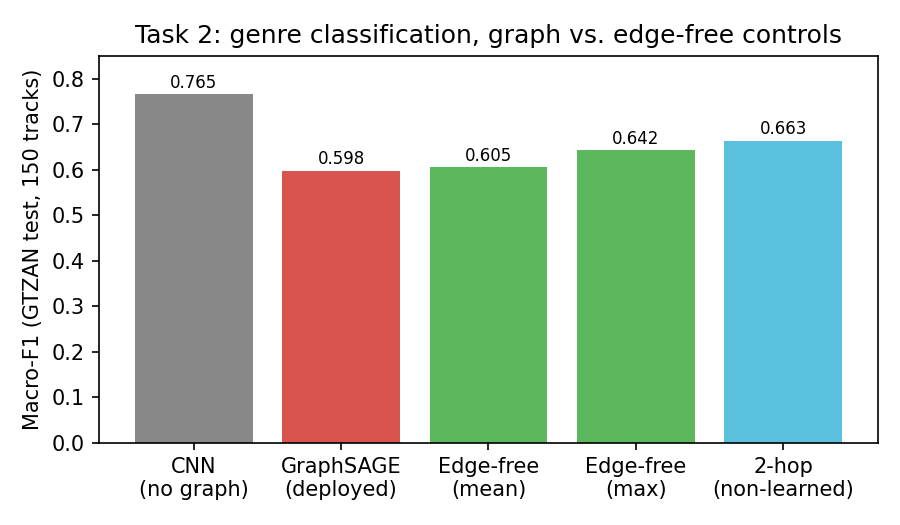
\includegraphics[width=0.8\columnwidth]{figures/fig2_task2_comparison.png}
\caption{Task 2: GTZAN genre classification, graph model vs.\ controls.}
\label{fig:task2}
\end{figure}
The pooling-matched comparison -- both models using mean-pool readout, the fairest single
comparison here -- has the edge-free encoder ahead by \textbf{+0.0072} macro-F1 (0.6049 vs.\
0.5976), using 47\% fewer parameters and no edge information (Figure~\ref{fig:task2}). Its
best result overall, at max-pool, is further ahead (+0.045), but that changes pooling as well
as topology and is not the clean ablation; we report it as the edge-free model's genuine best
result, not the fairest comparison -- neither reading has the graph model ahead. A separate,
repaired, sparser graph construction (mutual $k$-NN, three regimes, three poolings, 8 seeds
each, real vs.\ none/shuffled/random, 27 contrasts \cite{tismir_audit}) likewise found no
training-time contrast favoring the real graph; 18 of the 27 (real-vs-shuffled/random, same
architecture, changing only edge identity) are the topology-only evidence, the remaining 9
(real-vs-none) an edge-free comparison like this paper's own Task 2 control, not
double-counted here. Non-learned exact 2-hop aggregation also beats GraphSAGE, suggesting
part of the gap is GraphSAGE's learned aggregation under-using available signal, not only
weak topology -- a distinction we return to in Section~\ref{sec:discussion}.

\subsection{Task 3: does the graph complement text?}\label{sec:results-t3}
\begin{table}[t]
\centering
\caption{Task 3, MusicCaps fusion (715 test examples, except the edge-free row, which is
validation-only -- see note below).}
\footnotesize
\begin{tabular}{lccc}
\toprule
Mode & Macro-F1 & Micro-F1 & AUC-PR \\
\midrule
bert\_only & \textbf{0.7298} & 0.7647 & 0.7485 \\
gnn\_only (unweighted) & 0.0112 & 0.0290 & 0.0879 \\
gnn\_only (pos-weighted) & 0.1621 & 0.1839 & 0.1196 \\
edge-free gnn, pos-w.\ (max)$^{\dagger}$ & 0.1689 & -- & -- \\
concat & 0.7061 & 0.7478 & 0.7367 \\
cross\_attention & 0.6951 & 0.7398 & 0.7310 \\
\bottomrule
\end{tabular}

\vspace{2pt}
{\footnotesize $^{\dagger}$Validation set, not test -- see Section~\ref{sec:protocol}.}
\label{tab:task3-full}
\end{table}
Text alone (0.7298) outperforms every fusion mode; neither \textit{concat} (0.7061) nor
\textit{cross\_attention} (0.6951) improves on it. The edge-free \textit{gnn\_only} control
was only evaluated on validation, and its pooling-matched comparison does not repeat Task
2's pattern: at mean-pool (matching GraphSAGE's own pooling), the GraphSAGE-equivalent
baseline reaches 0.1640 against the edge-free encoder's 0.1599 -- the graph slightly
\emph{ahead} by +0.0041; only at max-pool does the edge-free encoder lead (0.1689). Both
edge-free readings share the GraphSAGE-equivalent comparator's positive-class weighting,
unlike the Table~\ref{tab:task3-full} rows discussed under Class Weighting
(Section~\ref{sec:protocol}). We report both honestly rather than quote only the max-pool
number: unlike Task 2's, this comparison does not show a clean edge-free advantage once
pooling is fixed, and we do not treat it as this task's primary evidence in either direction
-- that role belongs to the branch-zeroing and complementarity diagnostics below, both on the
real test set and unaffected by this pooling question.

\begin{figure}[t]
\centering
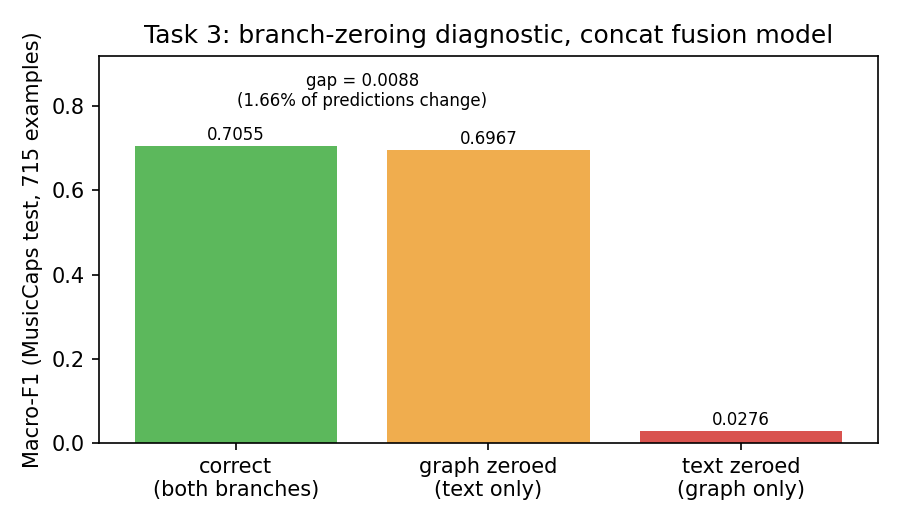
\includegraphics[width=0.8\columnwidth]{figures/fig3_task3_branch_zeroing.png}
\caption{Task 3: branch-zeroing diagnostic on the trained \textit{concat} fusion model.}
\label{fig:task3}
\end{figure}

\textbf{Branch-zeroing} (Figure~\ref{fig:task3}): replacing the
graph embedding with zeros inside the trained \textit{concat} model changes only
\textbf{1.66\%} of individual (example, tag) predictions and costs \textbf{0.0088} macro-F1
(0.7055 $\to$ 0.6967; 0.7055 is this diagnostic run's own re-measurement of \textit{concat},
negligibly different from Table~II's 0.7061); zeroing the text branch instead costs 0.6779
macro-F1, confirming text is overwhelmingly informative. This 0.0088 comes from the primary
evidence base (Section~\ref{sec:data}). The accompanying repository's own
\texttt{src/task3\_branch\_zeroing.py} instead reports 0.1205 (archived at
\texttt{results/task3\_branch\_zeroing.json}), against a \textit{concat} checkpoint that
repository's own training produced on its 673-example, 30-tag split -- a trained artifact not
itself shipped there, so a fresh clone cannot rerun this exactly without retraining, and
retraining is not guaranteed to reproduce 0.1205 given the non-determinism
Section~\ref{sec:discussion} discloses. Despite sharing this script's name, it runs a
different implementation, different data, and a differently trained checkpoint, part of a
disclosed follow-up that did not confirm this reading (Section~\ref{sec:discussion}) -- the
two numbers are not interchangeable, named explicitly rather than let the shared filename
imply otherwise.

\textbf{Complementarity}: cross-tabulating \textit{bert\_only} against \textit{gnn\_only}
predictions -- two separately-trained, single-branch models, not the fusion model
(35{,}750 cells, 715 examples $\times$ 50 tags) -- using the standard, unweighted
\textit{gnn\_only} checkpoint (macro-F1 0.0112) finds the graph model correct on 508 of
1{,}047 cells where text is wrong (\textbf{48.5\%}, an apparent "rescue rate"). Taken at face
value this looks like real, modest complementary signal. It is not: this checkpoint's
precision/recall (Table~\ref{tab:task3-full}) are exactly 0.0 for 45 of 50 tags -- it
predicts positive for only 5 -- so most "correct" cells are true negatives from never
predicting positive, not audio-based detection. Splitting the 508 by label polarity (the same
check applied to the accompanying repository's own numbers, Section~\ref{sec:discussion})
confirms this: only \textbf{3 of 508} (0.6\%) are genuine true positives where text was a
false negative; the remaining \textbf{505 of 508} (99.4\%) are the graph model defaulting to
"absent" while text wrongly said "present." An always-predict-absent classifier would, by
construction, rescue the same 509-of-1{,}047 (48.6\%) -- essentially the observed 48.5\%, so
this headline number does not distinguish the checkpoint from a trivial one and is not read
as complementary signal; it is also outnumbered by the reverse 1{,}735 cells where text is
right and the graph wrong. This cross-tabulation is correlational, comparing two
independently trained models. Branch-zeroing above is a narrower causal intervention: it
manipulates the trained fusion model's input at inference and measures the output effect,
distinct from a training-time test of a graph-absent-from-the-start model (zero may be an
input the model never saw, so this measures reliance as currently trained, not causal
contribution under retraining). With that scope, it found removing the graph costs only
0.0088 macro-F1 -- small, but genuine, a more direct kind of evidence than complementarity's
correlational count. One further, tentative point: richer pretrained node features (frozen
CNN embeddings trained for GTZAN genre, replacing chroma+MFCC) give a modest single-seed,
validation-only gain (0.1640 $\to$ 0.1846, +0.0206) -- a hint that node-feature weakness is
part of the story, but one run, a mismatched embedding source, no test-set or multi-seed
confirmation.

\subsection{Task 4: does any graph benefit survive under retrieval?}\label{sec:results-t4}
\begin{table}[t]
\centering
\caption{Task 4, MusicCaps retrieval (673 test examples), mean $\pm$ population standard
deviation (\texttt{ddof=0}) over 3 seeds.}
\begin{tabular}{lcc}
\toprule
Metric & Real graph & Edge-free \\
\midrule
Audio$\to$Text R@1  & 0.0124 $\pm$ 0.0019 & 0.0124 $\pm$ 0.0046 \\
Audio$\to$Text R@5  & 0.0570 $\pm$ 0.0062 & 0.0589 $\pm$ 0.0046 \\
Audio$\to$Text R@10 & 0.1025 $\pm$ 0.0053 & 0.1000 $\pm$ 0.0091 \\
Text$\to$Audio R@1  & 0.0099 $\pm$ 0.0031 & 0.0104 $\pm$ 0.0032 \\
Text$\to$Audio R@5  & 0.0515 $\pm$ 0.0037 & 0.0570 $\pm$ 0.0101 \\
Text$\to$Audio R@10 & 0.1030 $\pm$ 0.0125 & 0.1010 $\pm$ 0.0063 \\
\bottomrule
\end{tabular}
\label{tab:task4-full}
\end{table}
\begin{figure}[t]
\centering
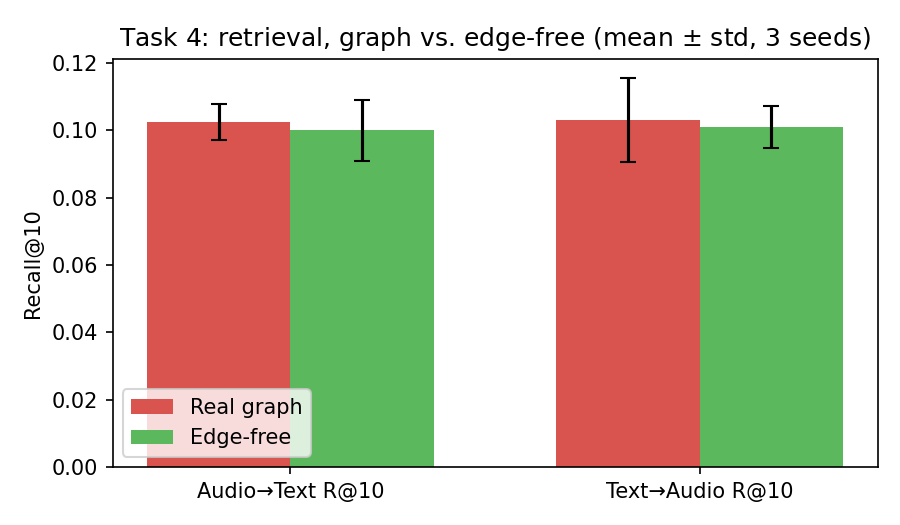
\includegraphics[width=0.8\columnwidth]{figures/fig4_task4_retrieval.png}
\caption{Task 4: retrieval Recall@10, graph vs.\ edge-free encoder.}
\label{fig:task4}
\end{figure}
Across three training seeds, the absolute difference between the real-graph and edge-free
encoders' means ranges from 0.00000 to 0.00545 across the six reported metrics
(Figure~\ref{fig:task4}) -- smaller, on every metric, than at least one condition's own
population standard deviation (ddof=0), though not always both, so we avoid the imprecise
"within one SD" description. With only three runs and no significance/equivalence test, the
defensible statement is no consistent advantage for either encoder in either direction, not
proof of equivalence. This is more informative than an earlier single-seed check, which
showed edge-free ahead on audio$\to$text R@10 by 0.028 and graph-based ahead on
text$\to$audio R@10 by 0.015 -- neither gap recurs in the three-seed rerun (per-seed gaps
range only $-0.013$ to $+0.021$ and $-0.006$ to $+0.010$ respectively, narrower in both
directions), though three seeds is too small a basis to call this an established difference
in variability, only a description of what these runs showed.
Zero-shot tag prediction (embedding tag names as text, no supervised classifier;
Section~\ref{sec:protocol}) reaches macro-F1 0.146 on the single seed-42 real-graph
checkpoint -- not the three seeds behind Table~\ref{tab:task4-full}, and without a
random-encoder control to confirm this is above chance, so we report it without the stronger
"confirms semantic content" claim it might otherwise support. It is, as expected, far below
Task 1's supervised classifier, for a system that never sees tag or genre labels during
training (it sees which caption pairs with which clip, a form of supervision, just not a
tag/genre label). In a separate, single-seed check on the real-graph encoder, quadrupling the
contrastive batch size (32$\to$128) changed R@10 by at most 0.006 in either direction --
suggestive against batch size being the bottleneck, though not repeated for the edge-free
encoder or across seeds, so a secondary observation, not a controlled result on the same
footing as the comparison above.

\textbf{Qualitative failure review.} A possible objection to exact-pair retrieval evaluation
is that a "wrong" top-1 result might still be semantically reasonable, just not the official
paired clip -- a false negative of the protocol, not a model error. We inspected 20
successes (true clip in the top 3) and 20 failures (below 10th) manually, comparing each
failure's query caption against its top-1 match's caption. The failures are not close
misses: median rank 166 of 673, ranging 28-352 across the 20 (individual ranks archived
alongside this evaluation). Reading the caption pairs, the large majority describe clearly
different instrumentation, genre, or mood (e.g.\ a piano-and-propeller query's top-1 match
was a Russian lullaby with vocals). A small number share a coarse category (both
instrumental, or reverb-heavy) without matching specific content. We do not find evidence
that exact-pair evaluation hides a large population of semantically-correct-but-unpaired
matches; most failures are genuine retrieval errors. Real limits: the 40 examples are the
first qualifying test cases in dataset order, not a random sample, judged by one author
without a blinded rater or predefined rubric -- a manual sanity check, not a formal
annotation study.

\section{Cross-Task Analysis}\label{sec:cross-task}

Individually, each task's result is one comparison, with its own caveats. Together, they form
a pattern worth examining directly, without overstating any single piece of it.

\textbf{The similarity graph is close to a deterministic function of its own node features.}
The similarity edges used throughout this paper are constructed as $A_{\mathrm{sim}}=g(X)$
for a fixed threshold rule $g$ (Section~\ref{sec:data}). Because $A_{\mathrm{sim}}$ is a
deterministic function of $X$ and nothing else, it cannot, in principle, carry information
about a downstream target $Y$ beyond what $X$ already carries:
$I(Y;X,A_{\mathrm{sim}})=I(Y;X)$, a direct instance of the data-processing inequality
\cite{cover2006elements}. This is a claim about Shannon information -- that a sufficiently
powerful model, trained without limit, could not extract more from $(X,A_{\mathrm{sim}})$
jointly than from $X$ alone -- not that any particular finite, trained model here reaches
that limit; the experiments, not this inequality alone, test whether the trained models
benefit in practice. This covers the similarity edges specifically, not the deployed
construction's temporal edges, which encode segment order and are not recoverable from an
unordered feature set. It is not only theoretical: the deployed graphs, for the two datasets
this paper's comparisons use, have mean edge density 95.4\%-97.9\%, with 76.4\%-84.0\% of
individual graphs fully connected, and randomly rewiring the edge set reproduces almost the
same graph under a different name (Section~\ref{sec:data}).

\textbf{The direct graph-vs-edge-free comparisons are mixed at the single-cell level, but
none shows the graph clearly ahead once its own best supporting diagnostic is considered.}
Task 2's pooling-matched comparison favors the edge-free encoder by +0.0072 macro-F1 (a
larger, pooling-confounded +0.045 gap also exists, reported separately,
Section~\ref{sec:results-t2}). Task 3's standalone edge-free \textit{gnn\_only} comparison is
genuinely mixed and pooling-dependent -- the graph-equivalent baseline is slightly ahead at
mean-pool (0.1640 vs.\ 0.1599) and behind at max-pool (0.1640 vs.\ 0.1689), both validation
scores (Section~\ref{sec:results-t3}) -- so we do not read this as evidence in either
direction; Task 3's more informative, test-set evidence is branch-zeroing and
complementarity -- branch-zeroing finds a small positive contribution (+0.0088 macro-F1, not
zero, just small), while complementarity, corrected for the graph-only checkpoint's
label-polarity collapse (Section~\ref{sec:results-t3}), finds essentially none. Task 4's
edge-free and graph-based encoders show no reliable difference across three seeds on any
metric (Section~\ref{sec:results-t4}). Taken together: no task shows a clear graph advantage
across the available test-set evidence -- Task 2's control has disclosed dropout and seed
mismatches (Section~\ref{sec:protocol}), Task 3's edge-free comparison is validation-only,
and Task 4 supplies the repeated test-set comparison; where a standalone comparison is mixed
or pooling-dependent (Task 3), we say so rather than select the reading that fits the
pattern.

\textbf{The correlational diagnostic finds essentially no complementary signal; the causal
diagnostic finds a small but genuine one.} These are two different diagnostics, not one, and do not need to agree in degree to agree in
spirit. Complementarity (Section~\ref{sec:results-t3}) is correlational: comparing two
independently trained, single-branch models, the graph-only model is correct on 508 of
1{,}047 cells where text is wrong, a 48.5\% headline "rescue rate." This is misleading: the
graph-only checkpoint has exactly 0.0 precision and recall on 45 of 50 tags, so splitting the
508 by label polarity shows only 3 (0.6\%) are genuine true positives; the other 505 of 508
(99.4\%) are the graph model defaulting to "absent" while text wrongly said "present" -- an
always-predict-absent classifier would rescue essentially the same 48.6\%, so this number
does not distinguish the checkpoint from a trivial one. Branch-zeroing is a within-checkpoint
inference-time intervention, not a correlational count: inside the trained fusion model,
removing the graph branch costs 0.0088 macro-F1 and changes 1.66\% of individual
predictions -- small, but real (Section~\ref{sec:results-t3} notes what this diagnostic does
and does not establish about training-time causation). The two are not in tension:
complementarity, properly read, finds only three positive-label rescues -- too few for
meaningful complementary detection; branch-zeroing finds the fusion model relies on the graph
branch -- topology and node features together, since zeroing removes both, not
topology-isolating -- only slightly, not not at all. They are not two measurements of the
same quantity: complementarity speaks to whether the independently-trained graph-only model
detects tags text misses (largely not), while branch-zeroing speaks to the trained fusion
model's own reliance (slight, but real, not topology-specific). We read them together only as
pointing the same direction here, not converging on one number -- and
Section~\ref{sec:discussion} reports that a second implementation found substantially greater
fusion-model reliance and substantially more genuine rescue, an unresolved disagreement we do
not paper over here.

\textbf{Text dominance and graph weakness are separate findings, not one explanation for the
other.} Caption text leaks a substantial fraction of target labels directly (69.1\%
label-macro-averaged lexical exposure, measured for Task 1), explaining part of Task 1's text
strength independent of the graph; the sanitization control measuring this precisely
(Section~\ref{sec:results}) was only run for Task 1, so we do not claim the same figure or
result for Task 3 -- Task 3 uses the same MusicCaps captions, so the same leakage channel
plausibly exists there too, but this was not separately measured. The graph's weakness is
established separately, by the edge-free controls, not inferred from text's strength. Both
are true at once, reported as two distinct findings.

\textbf{Dataset integrity is a genuine open question for the small comparisons, though not
for the largest ones.} The one confirmed leakage effect (GTZAN's 7 cross-split exact-duplicate pairs, 3 of 150 test
tracks affected, Section~\ref{sec:data}) is small relative to Task 2's CNN-vs-GraphSAGE gap
(0.168) and its own larger, pooling-confounded edge-free comparison (0.045); three memorized
tracks are unlikely to move either by that much. It is not demonstrably too small, however,
to matter for Task 2's smaller, pooling-matched gap (0.0072): macro-F1 can move more than a
raw accuracy count suggests when errors concentrate within one genre, and a duplicated
validation-split track can also affect which checkpoint is selected. We do not correct the
split and rerun Task 2 here -- that would change every Task 2 number and is left as a direct
next step -- so we state this as an unresolved caveat on the smallest comparison
specifically, not the pattern as a whole. A companion audit's repaired factorial
\cite{tismir_audit} repairs the \emph{graph construction} (a separate density defect,
unrelated to this leakage) and finds the same qualitative pattern, but reuses the same GTZAN
split, so it does \emph{not} escape this leakage caveat -- not claimed as leakage-free
corroboration. Task 4 adds a different kind of independence: it uses MusicCaps (checked clean
of split-level ID leakage, Section~\ref{sec:data}) and a completely different task type, so at
least one leg of the pattern does not share GTZAN's leakage risk at all.

\textbf{The pattern holds across three structurally different learning settings, though not
via the identical measurement in each.} Single-label classification (Task 2), multi-label classification with a strong second
modality present (Task 3), and ranking under a contrastive objective with no class labels
(Task 4) are three different problems, evaluated with three different metrics; we do not
claim one uniform comparison recurs across all three. Task 2's direct comparison favors
edge-free. Task 3's own comparison is mixed (Section~\ref{sec:results-t3}); what recurs is
not "edge-free ahead" but the same underlying conclusion -- little detectable graph
benefit -- reached via an inference-time intervention and a correlational diagnostic instead.
Task 4 shows no reliable difference either way. The consistent thread is the
\emph{conclusion} (no reliable graph benefit detected), not an identically-shaped comparison,
more informative than any one task alone but read with the caveats above (validation-only
numbers and a mixed standalone result in Task 3, unresolved leakage for Task 2's smallest
comparison, two separate implementations across Tasks 1--3 versus Task 4) -- a consistent
signal, not four independent, airtight proofs of the same fact.

\section{Discussion}\label{sec:discussion}

\textbf{What this shows.} Across three tasks with different objectives, loss functions, and
evaluation metrics, we could not detect a reliable benefit from this system's
similarity-based audio graph beyond what its own node features already provide -- though the
evidence differs by task, not uniform. Task 2's pooling-matched comparison favors the
edge-free encoder directly. Task 3's own standalone comparison is mixed and pooling-dependent
and is \emph{not} the evidence we rely on there; its branch-zeroing and complementarity
diagnostics, both on held-out test data, establish two different, narrower things: branch-
zeroing shows the trained fusion model relies only slightly on the graph branch (topology and
node features together, since zeroing removes both -- not topology-isolating), and
complementarity shows the independently-trained graph-only model detects almost nothing text
misses (a claim about that model, not the fusion model). Together, in this evidence base,
they point to little demonstrated graph value for Task 3 -- a follow-up check later in this
section found the opposite in a second implementation, unresolved which reading generalizes.
Task 4 shows no reliable difference across three seeds. Tasks 2 and 4 rely on
width/depth-matched, lower-parameter edge-free controls; Task 3's such control is
validation-only, so its test-set evidence comes from branch-zeroing and complementarity
instead, neither an edge-free-encoder comparison. The three findings are not built from one
identical comparison type, stated at each step rather than only here.

\textbf{What this does not show.} It does not show that graph neural networks are a poor
choice for music understanding in general, or that no graph construction could help this
kind of system -- only that \emph{this specific} feature-induced similarity graph, applied to
\emph{these} node features, on \emph{these} datasets, gave the model little it did not
already have. A graph built from a genuinely external relation -- not recomputable from the
same node features, such as annotated chord progressions, beat structure, or section
repetition -- is not ruled out and remains untested here.

\textbf{Why this might be happening, and a genuine complication.} The clearest candidate
explanation is structural: a similarity threshold applied to the same features used as node
content produces an adjacency matrix that is, information-theoretically, redundant with those
features (Section~\ref{sec:cross-task}). A secondary, speculative possibility: the limited
topology present is not fully exploited by the trained GraphSAGE model -- the broader GNN
literature separately finds trained message-passing layers can under-use structure through
over-smoothing \cite{li2018oversmoothing}, and a fixed propagation step can match or exceed a
trained GCN-style layer \cite{wu2019sgc}. Table \ref{tab:task2-full}'s exact 2-hop result
(0.6630, beating both edge-free numbers and GraphSAGE, not the CNN baseline at 0.7654) is a
genuine complication for a "topology never helps" reading, reported rather than explained
away -- but not a clean ablation: the 2-hop pipeline uses full-batch Adam, 200 epochs, no
dropout, while GraphSAGE's script does not pass its configured dropout through and trains at
the default 0.2 (Section~\ref{sec:protocol} discloses this bug precisely), with mini-batches
and early stopping (both share weight decay $10^{-4}$). These recipe differences, not only
whether aggregation is learned, could account for some or all of the gap, so we treat it as
exploratory -- a cleaner, topology-only result exists in a companion audit
\cite{tismir_audit} (Section~\ref{sec:results-t2}), a same-architecture
real/shuffled/random-edge factorial, but we flag rather than lean on it: it is an
unpublished, anonymized-for-review manuscript with no stable public identifier at writing,
cited rather than reproduced, its methods and tables not included alongside this paper or
independently inspectable here. We lack an equivalent 2-hop control for Tasks 3/4, and this
result is single-run despite sharing GraphSAGE's seed (42); porting its script into this
repository (\texttt{task2\_exact\_2hop\_control.py}) also found it not exactly reproducible
across environments -- an independent rerun with identical code, seed, and data reached
0.6551, not 0.6630, plausibly floating-point non-associativity in the accumulation step. Both
values still clearly exceed GraphSAGE (0.5976) and both edge-free readings (0.6049, 0.6425),
not changing the qualitative finding, but a further reason to treat this result as
exploratory. We do not treat it as overturning the paper's pattern -- but it keeps this paper
from concluding the deployed encoders extract everything the node features offer.

\textbf{Limitations.} The caption-sanitization control (69.1\% lexical exposure, 84.3\%
retention after retraining, Section~\ref{sec:data}) was run in an internal research directory
outside the two implementations this paper draws from; the stored numbers were directly
re-verified against their result files, but the training script itself is not included
alongside this paper, a reproducibility gap disclosed here rather than left implicit. Task 2
and Task 3's main comparisons use a single training seed each; only Task 4's headline
comparison repeats across seeds. GTZAN carries a small, previously undocumented amount of
exact-duplicate, cross-split leakage (Section~\ref{sec:data}); MusicCaps was checked clean at
the ID level but not audio-content level, so duplicate underlying recordings, if any, would
not have been caught. Neither dataset's artist-level leakage could be checked, since neither
ships usable artist metadata. This paper uses the original, denser graph construction
throughout (Section~\ref{sec:data}); a companion audit of the same system repairs this
construction and finds the same qualitative pattern on repaired graphs \cite{tismir_audit},
but this paper's own four-task comparisons were not rerun on it. Retrieval evaluation here
treats only the one official caption as correct; a semantically reasonable but unpaired clip
would be scored as an error. We checked this directly on 20 retrieval failures
(Section~\ref{sec:results-t4}) and did not find evidence of a large hidden population of such
cases -- most failures were genuine mismatches, the true clip ranked far outside the top 10.
This used only one checkpoint, 20 non-randomly-selected examples, and one unblinded rater
with no predefined rubric, so it does not rule out the effect entirely, only that it is not
large enough to be obvious on a direct look.

\textbf{A follow-up check that complicates the Task 3 finding, and what we do and do not know
about why.} We reran Task 3's branch-zeroing and complementarity diagnostics in a second,
independent implementation of this same architecture family -- the one Task 4's own numbers
are drawn from -- and got a different answer. Removing the graph branch there costs 0.12
macro-F1 at that implementation's own epoch budget and 0.1672 when retrained at the shorter
budget used before (a single archived run; we did not force deterministic training, so, as
with Table~\ref{tab:task2-full}'s 2-hop result, an exact rerun could land differently; no
additional runs were archived to quantify that); complementarity finds 169 of 359 rescued
cells (47.1\%) genuine at the longer budget and 142 of 427 (33.3\%) at the shorter, both well
above the 3 of 508 (0.6\%) reported above. Both readings are real measurements, needing an
explanation rather than a choice of which to believe. The larger effect persists at the
shorter budget, so the longer budget alone does not explain the disagreement. One plausible
contributor is class weighting: unlike this section's complementarity checkpoint (trained
without positive-class weighting, collapsed to predicting a tag present for only 5 of 50),
the second implementation weights all four fusion modes, including \textit{gnn\_only},
throughout. We have not isolated weighting as the cause: the implementations also differ in
split size, tag vocabulary (50 here, 30 there), and segment length, and no
weighted-vs-unweighted comparison was run within one implementation to separate weighting
from these. In the second implementation, branch-zeroing found substantially greater
fusion-model reliance and complementarity substantially more genuine rescue by its own
graph-only model; neither isolates topology specifically, since branch-zeroing does not
separate topology from node information and complementarity is a statement about a separate
model, not the fusion model's behavior. We report this as an open, only partly explained
disagreement, not a correction to the numbers above and not evidence the graph helps once
weighted correctly.

\textbf{Why richer relations might behave differently.} A relation that is not a function of
the node features -- for example, which segments belong to the same repeated section, or
which two chords typically follow one another -- would fall outside the redundancy argument
in Section~\ref{sec:cross-task} by construction, since it encodes something the feature
vectors alone cannot recover. Testing this is a natural next step, not attempted here beyond
the informal argument above.

\section{Conclusion}

For similarity edges, Shannon redundancy with the node features follows analytically from
the construction, not from any experiment. What we tested, rather than assumed, is the
practical question -- whether this similarity-based audio graph nevertheless helps a real,
finite model -- across four tasks spanning text-only prediction, graph-only classification,
multimodal fusion, and cross-modal retrieval. Tasks 2 and 4 include a
direct, test-set graph-vs-edge-free comparison; Task 3's own such comparison is
validation-only, so its evidence instead comes from two test-set diagnostics: branch-zeroing
inside the trained fusion model, and a cross-tabulation of independently-trained
single-branch checkpoints. No \emph{learned-aggregation} graph-based model ever
showed a clear advantage over its edge-free alternative, and it trailed in Task 2's
pooling-matched reading -- a single-run difference, with GTZAN's small unresolved leakage
caveat and no uncertainty estimate, so we call this a trailing result, not a statistically
established loss.

One qualifier matters here. Task 2's non-learned exact 2-hop control, whose aggregation is
fixed rather than trained, does clearly beat every edge-free number -- a genuine complication,
discussed in Section~\ref{sec:discussion}, not swept into "graph-based model" for
convenience. Task 3's own standalone comparison was mixed and inconclusive on its own; in this
evidence base, branch-zeroing and complementarity -- an inference-time intervention on the
trained fusion model, and a correlational comparison of two separately-trained single-branch
models, respectively -- both point to little graph reliance instead. Section~\ref{sec:discussion}
also reports that the same two diagnostics, run against a second implementation's own
checkpoints, found substantially more reliance -- an unresolved disagreement between
implementations, not a second confirmation of the first. Task 4 showed no consistent advantage either way across three
seeds; with only three runs and no formal equivalence test, that is an absence of detected
difference, not proof of none.

We report the resulting conclusion as the paper's central finding: no task in this study
showed a clearly established graph advantage, though the supporting evidence and its strength
differ by task and are stated precisely rather than smoothed into one uniform result.
Presence of a graph branch in a music-understanding pipeline is not the same as demonstrated
reliance on it -- the two should be checked separately, not assumed to go together.


{\small
\bibliographystyle{IEEEtran}
\bibliography{references}
}

\end{document}
